\documentclass[a4paper,11pt]{jreport}

\usepackage[dvipdfmx]{graphicx}
\usepackage[dvipdfmx,bookmarks=true,bookmarksnumbered=true,bookmarkstype=toc,colorlinks=true,linkcolor=blue,citecolor=red]{hyperref}
\usepackage{pxjahyper}
\usepackage{ulem}
\usepackage{times} % use Times font instead of default one
\usepackage{amsmath,amsfonts}
\usepackage{bm}
\usepackage{url}
\usepackage{ascmac}
\usepackage{caption}
\usepackage{tabularx}

\setcounter{tocdepth}{3}
\setcounter{page}{-1}

\setlength{\oddsidemargin}{0.1in}
\setlength{\evensidemargin}{0.1in} 
\setlength{\topmargin}{0in}
\setlength{\textwidth}{6in} 
\setlength{\parskip}{0em}
\setlength{\topsep}{0em}

\usepackage{coins-jp}

\title{大規模言語モデルの性能評価を目的とした\\[2mm]
文脈情報に基づく日本語評価データの自動生成}
\author{佐多 亮明}
\advisor{山本 幹雄, 乾 孝司, 津川 翔}

\fiscalyear{2026}

\begin{document}
\maketitle
\thispagestyle{empty}
\newpage

\thispagestyle{empty}
\vspace*{20pt plus 1fil}
\parindent=1zw
\noindent
\begin{center}
{\Large \bf 要  旨}
\vspace{2cm}
\end{center}
近年、大規模言語モデル(LLM)は急速な発展を遂げているが、その性能を客観的に評価するための日本語の高品質な評価データセット(ベンチマーク)は不足している。従来の人手によるデータセット構築は、品質は高いものの、膨大な時間とコストを要するため、LLMの発展速度に追いつけないという課題がある。この問題を解決するため、LLM自身に評価データを自動生成させるアプローチが期待されているが、LLMが事実に基づかない情報を生成する「ハルシネーション」が、生成データの信頼性を損なうという新たな課題を生んでいる。

本研究では、このハルシネーションを抑制し、信頼性の高い日本語評価データを低コストかつスケーラブルに自動生成する手法を提案する。提案手法では、Wikipedia記事のような信頼できる「文脈」に事実を基づかせる(Fact-Grounded)ことで、ハルシネーションを抑制する。具体的な手法として、人間が作成した高品質な読解データセットであるJSQuADの入出力構造を意図的に組み替え、QAペア生成に特化したモデルを「指示チューニング」によって学習させる。

本手法の有効性を検証するため、自動生成したテストデータセットが、人間製ベンチマークと同様の評価軸として機能するかを実験的に評価した。評価指標には、複数のLLMの性能ランキングの一致度を測るスピアマンの順位相関係数($\rho$)を用いた。実験の結果、提案手法である指示チューニングは、Zero-Shot推論やFew-Shot推論といったベースライン手法を大幅に上回り、人間製ベンチマークと極めて高い相関($\rho = 0.8741$)を示すことを実証した。

本研究の成果は、低コストで信頼性の高い日本語評価データセットの持続的な供給手法を確立するものであり、今後の日本語LLMの研究開発エコシステムの発展に貢献することが期待される。

\par
\vspace{0pt plus 1fil}
\newpage

\pagenumbering{roman}
\tableofcontents
\listoffigures
\listoftables

\pagebreak \setcounter{page}{1}
\pagenumbering{arabic}

\chapter{序論}
\label{chap:introduction}

\section{背景と目的}
近年、大規模言語モデル(LLM)は、OpenAIのGPTシリーズ\cite{GPT-3}やGoogleのGeminiシリーズに代表されるように急速な発展を遂げており、その応用範囲は社会の多岐にわたる。この技術の健全な発展のためには、各モデルの能力を正確に理解し、比較するための信頼性の高い評価手法が不可欠である。しかし、特に日本語ドメインにおいては、モデルの性能を多角的に測定するための高品質な評価データセット(ベンチマーク)が、英語圏に比べて不足しているという課題が存在する\cite{Okazaki:COLM2024}。

従来、こうした評価データセットは人手によるアノテーションを通じて作成されてきた。このアプローチは品質を担保する上でのゴールドスタンダードであるが、膨大な時間と金銭的コストを要するという大きな制約を抱えている。結果として、次々と登場する新しいモデルの開発スピードに、評価データセットの整備が追いつかないという事態が生じている。

このコストと時間の問題を解決する有望な代替案として、LLM自体に評価データを自動生成させるアプローチが考えられる。しかし、この手法には「ハルシネーション(幻覚)」という重大な課題がつきまとう。これは、LLMが学習データに含まれない、あるいは事実に基づかない情報を、もっともらしく生成してしまう現象である。信頼できる情報源なしにデータを生成させると、内容が不正確であったり、問題として成立していなかったりする質の低いデータが大量に作られてしまう。さらに、一度生成されたデータに含まれるハルシネーションを事後的に高精度で検出し、除去することは極めて困難であり、生成されたデータの信頼性を保証する上での大きな障壁となっている。したがって、ハルシネーションを含むデータセットは信頼できる評価軸として機能せず、本末転倒となる。

そこで本研究では、生成プロセスそのものでハルシネーションを抑制し、事実に基づいた高品質な評価データを自動生成する手法の確立を目的とする。具体的には、Wikipedia記事のような信頼できる「文脈(コンテキスト)」をLLMに与え、そのテキスト内容に完全に準拠した一問一答形式の評価データを生成させる。そして、この手法で生成した評価データセットが、人手で作成された既存のベンチマークと同様に、様々なLLMの性能序列を正確に反映できるかを実証する。これにより、低コストかつ大規模な評価データセットの持続的な供給を可能にし、日本語LLMの研究開発エコシステムの発展に貢献することを目指す。

\section{本論文の構成}
本論文の構成は以下の通りである。第2章で本研究の基盤技術である大規模言語モデルの概要を述べる。第3章では、本研究で中核的に利用するデータセットについて説明する。第4章では関連研究を整理し、第5章で提案手法を詳述する。第6章では実験内容と結果、そして考察を述べ、第7章で結論と今後の展望をまとめる。






\chapter{大規模言語モデル}
\label{chap:llm}
本章では、本研究の対象である大規模言語モデル(LLM)について、その概要、アーキテクチャ、および学習方法といった基本的な枠組みを、サーベイ論文\cite{LLMSurvey}を基に解説する。

\section{LLMの概要と定義}
大規模言語モデル(LLM)とは、膨大なテキストデータを用いて学習された、非常に大規模なパラメータ数を持つニューラルネットワークモデルである。その最大の特徴は、特定のタスクに限定されず、多様な自然言語処理タスクを遂行できる汎用性にある\cite{LLMSurvey}。この能力は、モデルの規模(パラメータ数)、学習データサイズ、総計算量を増大させると、性能が予測可能に向上するという「スケーリング則(Scaling Laws)」によって支えられている\cite{LLMSurvey}。

また、モデルの規模が一定の閾値を超えると、小規模なモデルでは見られなかった新しい能力が発現することが知られており、これは「創発的能力(Emergent Abilities)」と呼ばれる\cite{LLMSurvey}。代表的な創発的能力には、少数の例示からタスクを遂行する文脈内学習(in-context learning)や、複雑な推論を中間ステップに分解する思考の連鎖(Chain-of-Thought)などが含まれる。

\section{主要なアーキテクチャ}
現代の主要なLLMは、そのほとんどがVaswaniらによって提案されたTransformerアーキテクチャ\cite{Transformers}を基盤としている。Transformerの核心は、Self-Attention(自己注意機構)と呼ばれるメカニズムにある。これは、入力されたテキスト系列内の各単語について、他のすべての単語との関連性の重みを計算し、文脈に応じた単語の表現を獲得する仕組みである。従来の再帰型ニューラルネットワーク(RNN)などと比較して、長い系列の依存関係を効率的に捉えることができ、また計算の並列化が容易であるため、大規模なデータとモデルの学習に適している\cite{LLMSurvey}。

Transformerを基盤とするLLMのアーキテクチャは、主に以下の3種類に分類される\cite{LLMSurvey}。
\begin{itemize}
    \item \textbf{Causal Decoder (Decoder-Only):} GPTシリーズ\cite{GPT-3}に代表される、単方向の自己注意機構を持つアーキテクチャ。ある時点の単語はそれ以前の単語にしか注意を払わないため、テキストの続きを予測する「次単語予測」タスクに自然な形で適用できる。この性質から、多くの生成系LLMで採用されている。
    \item \textbf{Encoder-Decoder:} 翻訳モデルなどで広く用いられてきた、入力を符号化するEncoderと、出力を生成するDecoderから成るアーキテクチャ。T5\cite{T5}などがこれにあたる。
    \item \textbf{Prefix-Decoder:} 上記2つを組み合わせたハイブリッドな構造を持つ。
\end{itemize}
本研究で扱うLLMは、主としてCausal Decoderアーキテクチャに分類されるものである。

\section{学習方法}
LLMの学習プロセスは、モデルに汎用的な言語能力を付与する「事前学習(Pre-training)」と、特定の目的や人間の意図に沿うようにモデルを適応させる「事後学習(Post-training)」の二段階に大別される。

\subsection{事前学習 (Pre-training)}
事前学習は、Web上のテキストや書籍といった大規模かつ多様なラベルなしコーパスを用いて行われる、自己教師あり学習のプロセスである。このアプローチの有効性は、Radfordらが最初のGPT(Generative Pre-trained Transformer)で示した\cite{GPT-1}、生成的な事前学習とそれに続く識別的なファインチューニングという2段階の学習パラダイムに端を発する。

事前学習における目的関数は、一般的に言語モデリング(Language Modeling)が用いられる。具体的には、あるコーパス$U = \{u_1, \dots, u_n\}$が与えられたとき、モデルは以下の対数尤度を最大化するように学習される。
$$
L_1(U) = \sum_i \log P(u_i | u_{i-k}, \dots, u_{i-1}; \Theta)
$$
ここで、$k$は文脈ウィンドウのサイズ、$\Theta$はニューラルネットワークのパラメータである。この「次単語予測」タスクを大規模なデータで解き続けることで、モデルは文法や事実知識、ある程度の推論能力といった、言語に関する汎用的で基礎的な能力を獲得する。この事前学習段階が、LLMの汎用性の源泉となっている。

\subsection{事後学習 (Post-training)}
事後学習は、事前学習によって汎用的な能力を獲得したモデルを、特定の目的や人間の意図に沿うように追加学習させるプロセスである。本研究に関連する主要な手法として、指示チューニングと人間からのフィードバックによる強化学習が挙げられる。

\subsubsection{指示チューニング (Instruction Tuning)}
指示チューニングは、Weiらによって提案された\cite{Instruction-Tuning}、LLMの能力を飛躍的に向上させた重要な技術の一つである。このアプローチの根底には、BrownらがGPT-3で示した「文脈内学習(in-context learning)」の概念がある\cite{GPT-3}。文脈内学習とは、モデルの重みを更新(ファインチューニング)することなく、推論時にプロンプトとして少数のタスク例(デモンストレーション)を与えるだけで、モデルがそのタスクを遂行する能力を指す。この能力は、図\ref{fig:gpt3_example}に示すように、与える例の数に応じて「ゼロショット」「ワンショット」「フューショット」として区別され、特にモデルの規模が大きくなるほど、文脈内の例からタスクを学習する効率が劇的に向上することが示された。

\begin{figure*}[t]
  \centering
  % 画像ファイル "gpt3_fig2.jpg" を "fig" フォルダ内に配置してください
  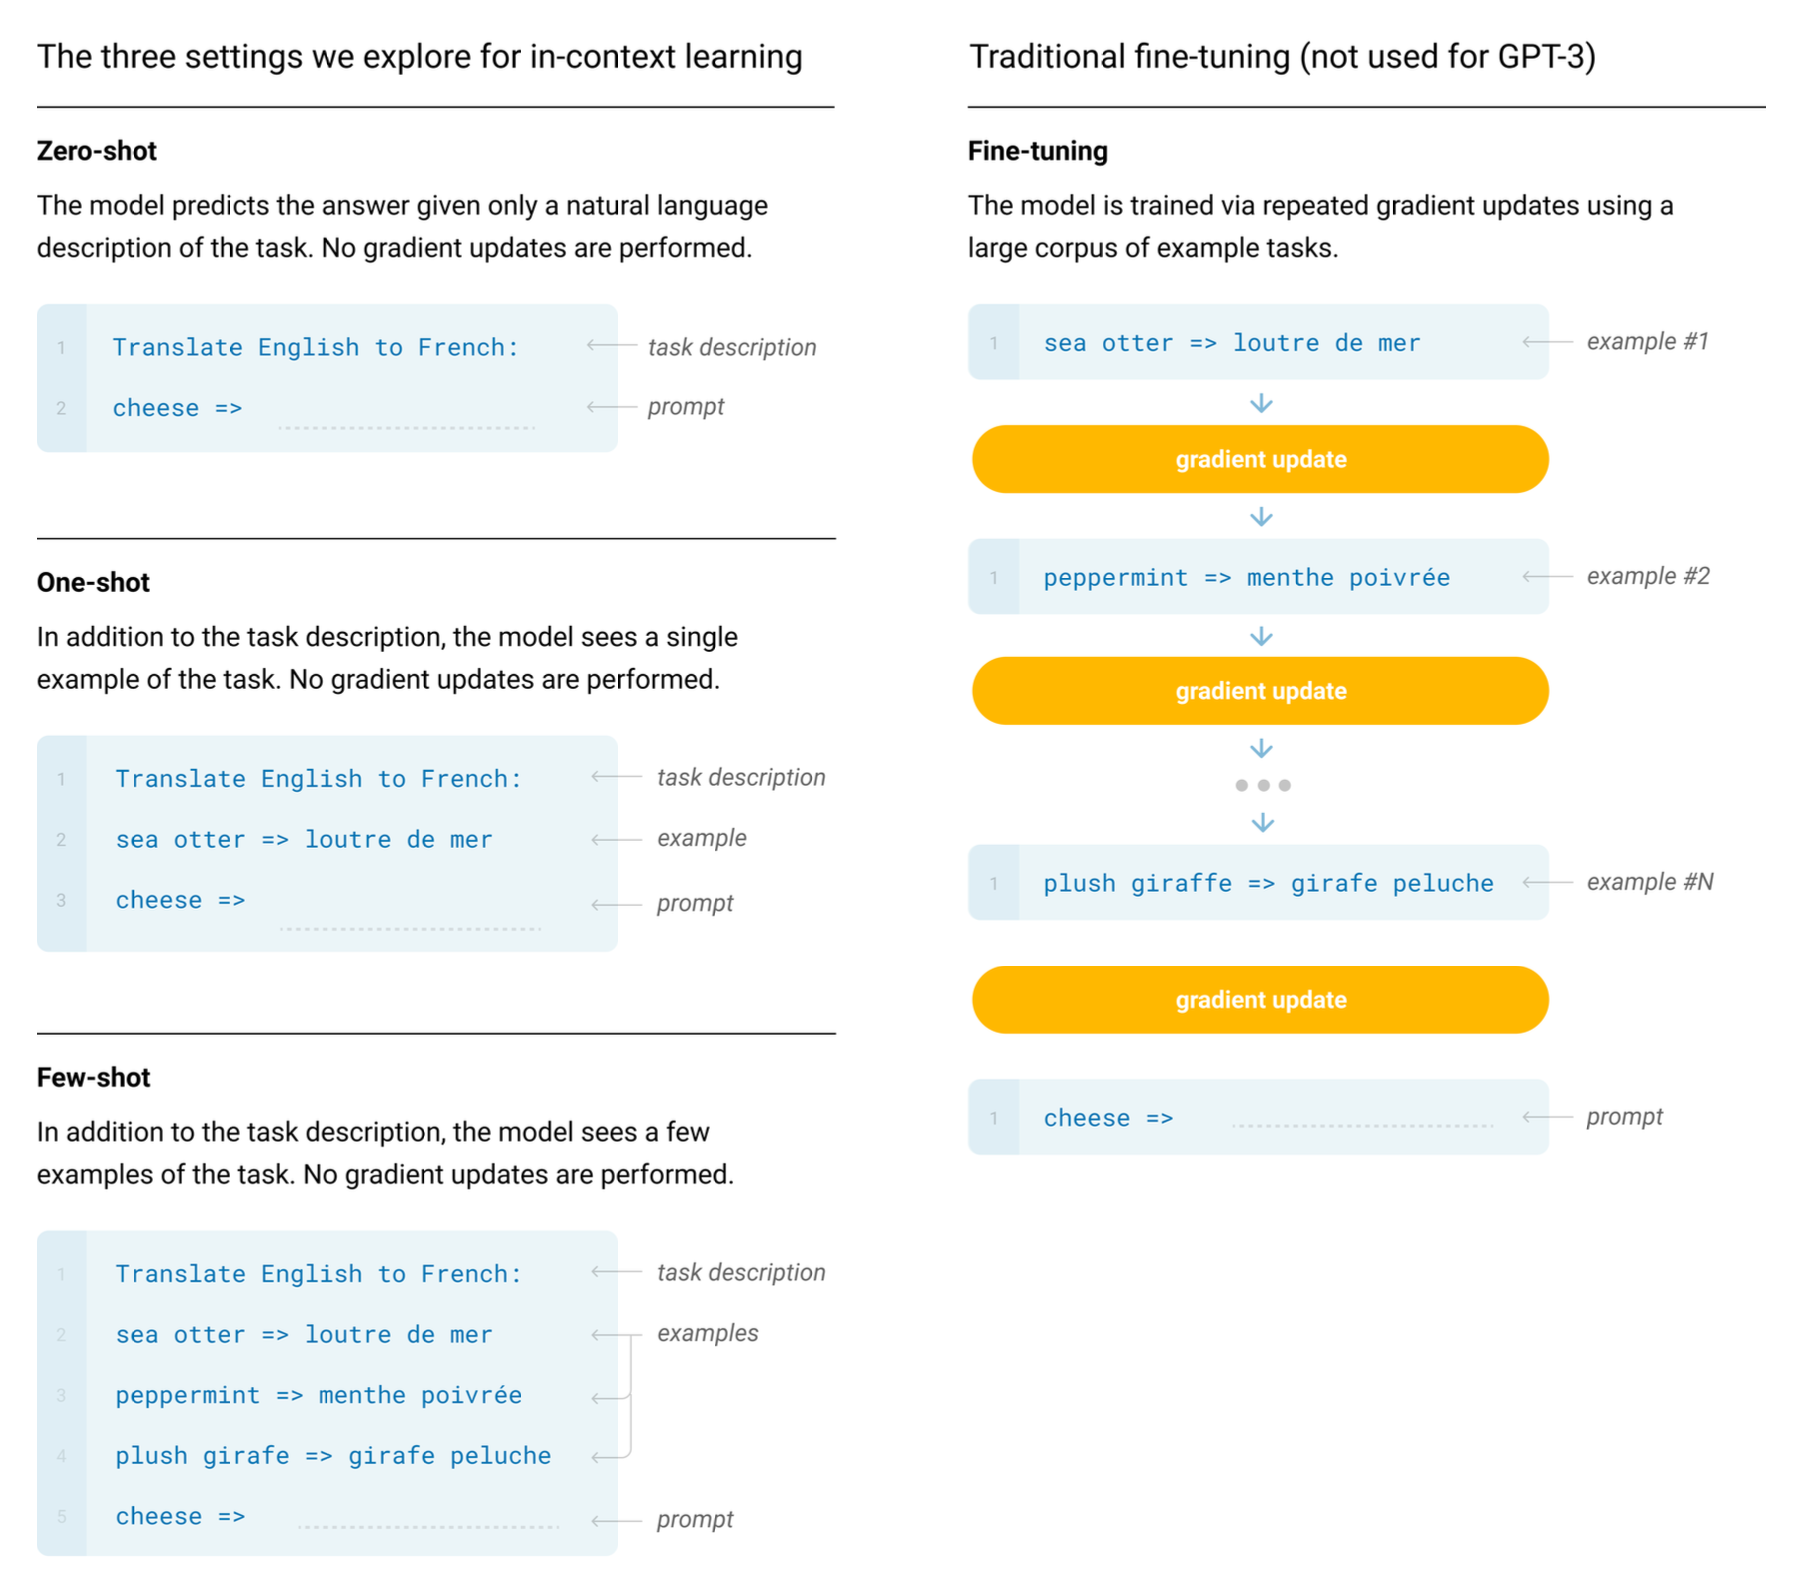
\includegraphics[width=0.9\linewidth]{./fig/gpt3_fig2.png}
  \caption{zero-shot, one-shot, few-shotとfine-tuningの違い\cite{GPT-3}}
  \label{fig:gpt3_example}
\end{figure*}

しかし、GPT-3のような大規模モデルでも、ゼロショット性能はフューショット性能に比べて著しく低いという課題があった。この課題を解決するために、Weiらによって提案されたのが「指示チューニング(Instruction Tuning)」である\cite{Instruction-Tuning}。これは、事前学習済みの言語モデルを、自然言語の「指示」として記述された、多数の既存データセットの集合でファインチューニングする手法である。このプロセスでは、入力トークン系列$x = \{x^1, \dots, x^m\}$と正解ラベル$y$からなる教師ありデータセット$C$を用いて、以下の対数尤度を最大化するようにモデルを微調整する。
$$
L_2(C) = \sum_{(x,y) \in C} \log P(y | x^1, \dots, x^m)
$$
ここで、$x$はタスクを説明する指示とタスクの入力を組み合わせたものであり、$y$はモデルが生成すべき正解の出力である。Weiらは、翻訳、質問応答など60以上の多様なNLPタスクを用いてこの学習を行い、その結果得られたモデルをFLAN (Finetuned Language Net)と名付けた。図\ref{fig:flan_example}にその概念図を示す。

\begin{figure*}[t]
  \centering
  % 画像ファイル "flan_fig2.png" を "fig" フォルダ内に配置してください
  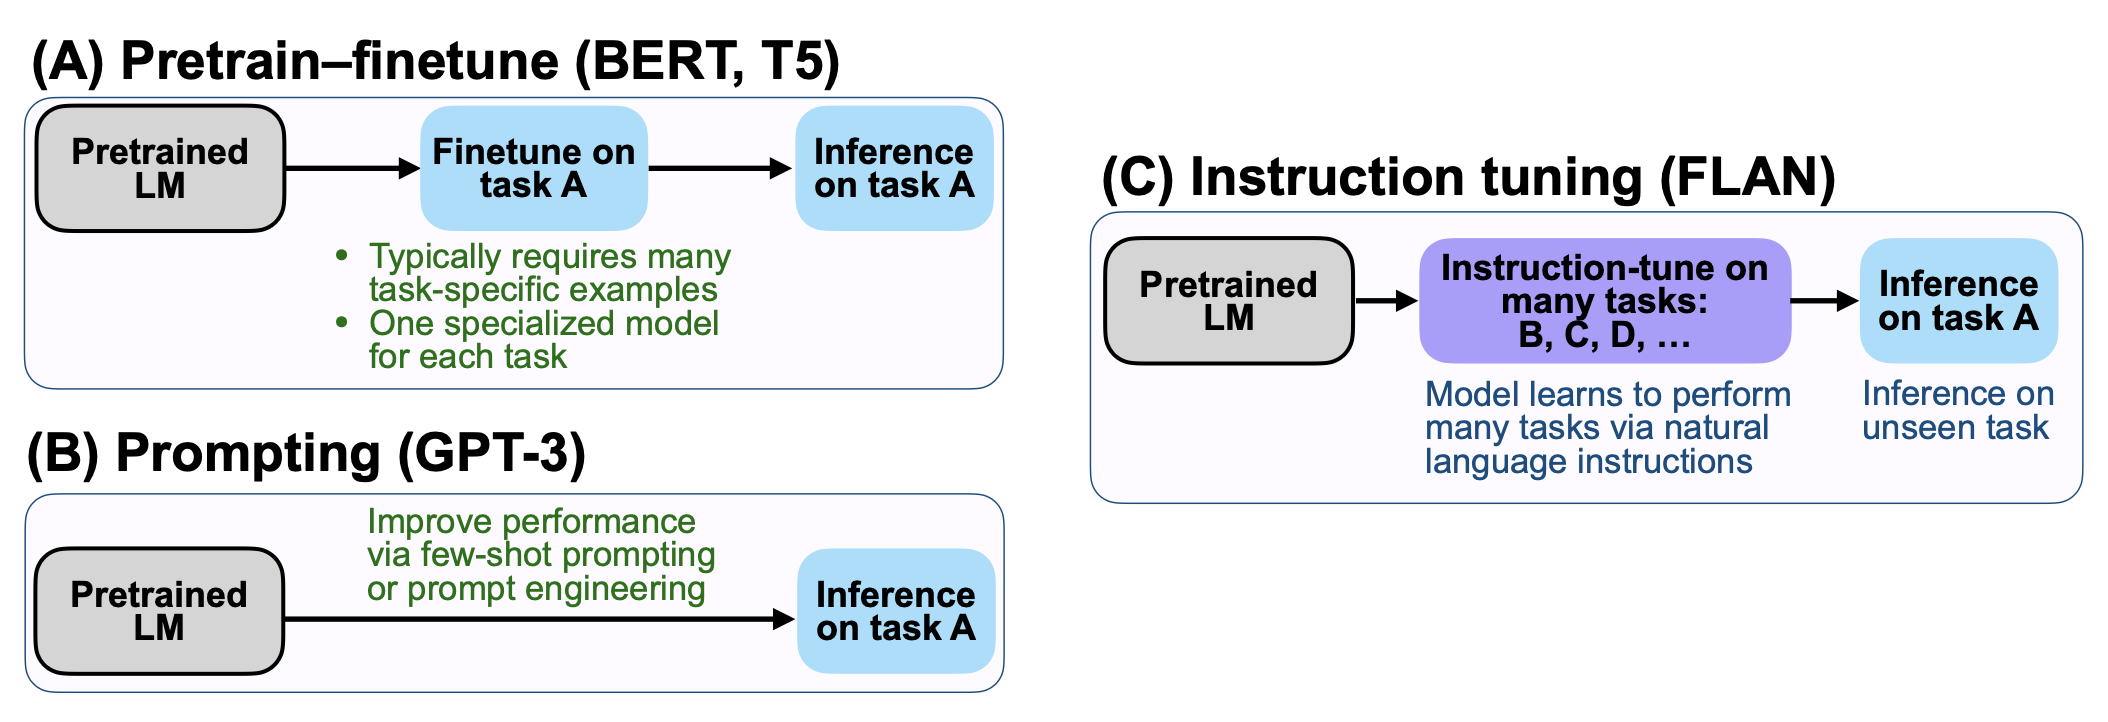
\includegraphics[width=0.9\linewidth]{./fig/flan_fig2.png}
  \caption{FLANの指示チューニングの例\cite{Instruction-Tuning}}
  \label{fig:flan_example}
\end{figure*}

指示チューニングの最大の成果は、学習時には見せていない「未知のタスク」に対するゼロショット性能を大幅に向上させた点にある。論文中のアブレーションスタディにより、この成功の鍵は「モデルの規模」と、学習に用いる「タスクの数と多様性」であることが明らかにされている。

\subsubsection{人間からのフィードバックによる強化学習 (RLHF)}
指示チューニングがモデルにタスクを遂行する能力を付与する一方で、その応答が人間の意図や価値観と一致しているかを保証するものではない。この課題に対し、LLMの挙動をより人間の好みに合致させるためのアライメント技術として、RLHF(Reinforcement Learning from Human Feedback)が提案された\cite{InstructGPT}。この手法は、特にInstructGPTやChatGPTといったモデルの成功を支える中核技術として知られている。

RLHFのプロセスは、図\ref{fig:rlhf_process}に示すように一般的に3つのステップで構成される\cite{InstructGPT}。

\begin{figure*}[t]
  \centering
  % 画像ファイル "rlhf_fig2.jpg" を "fig" フォルダ内に配置してください
  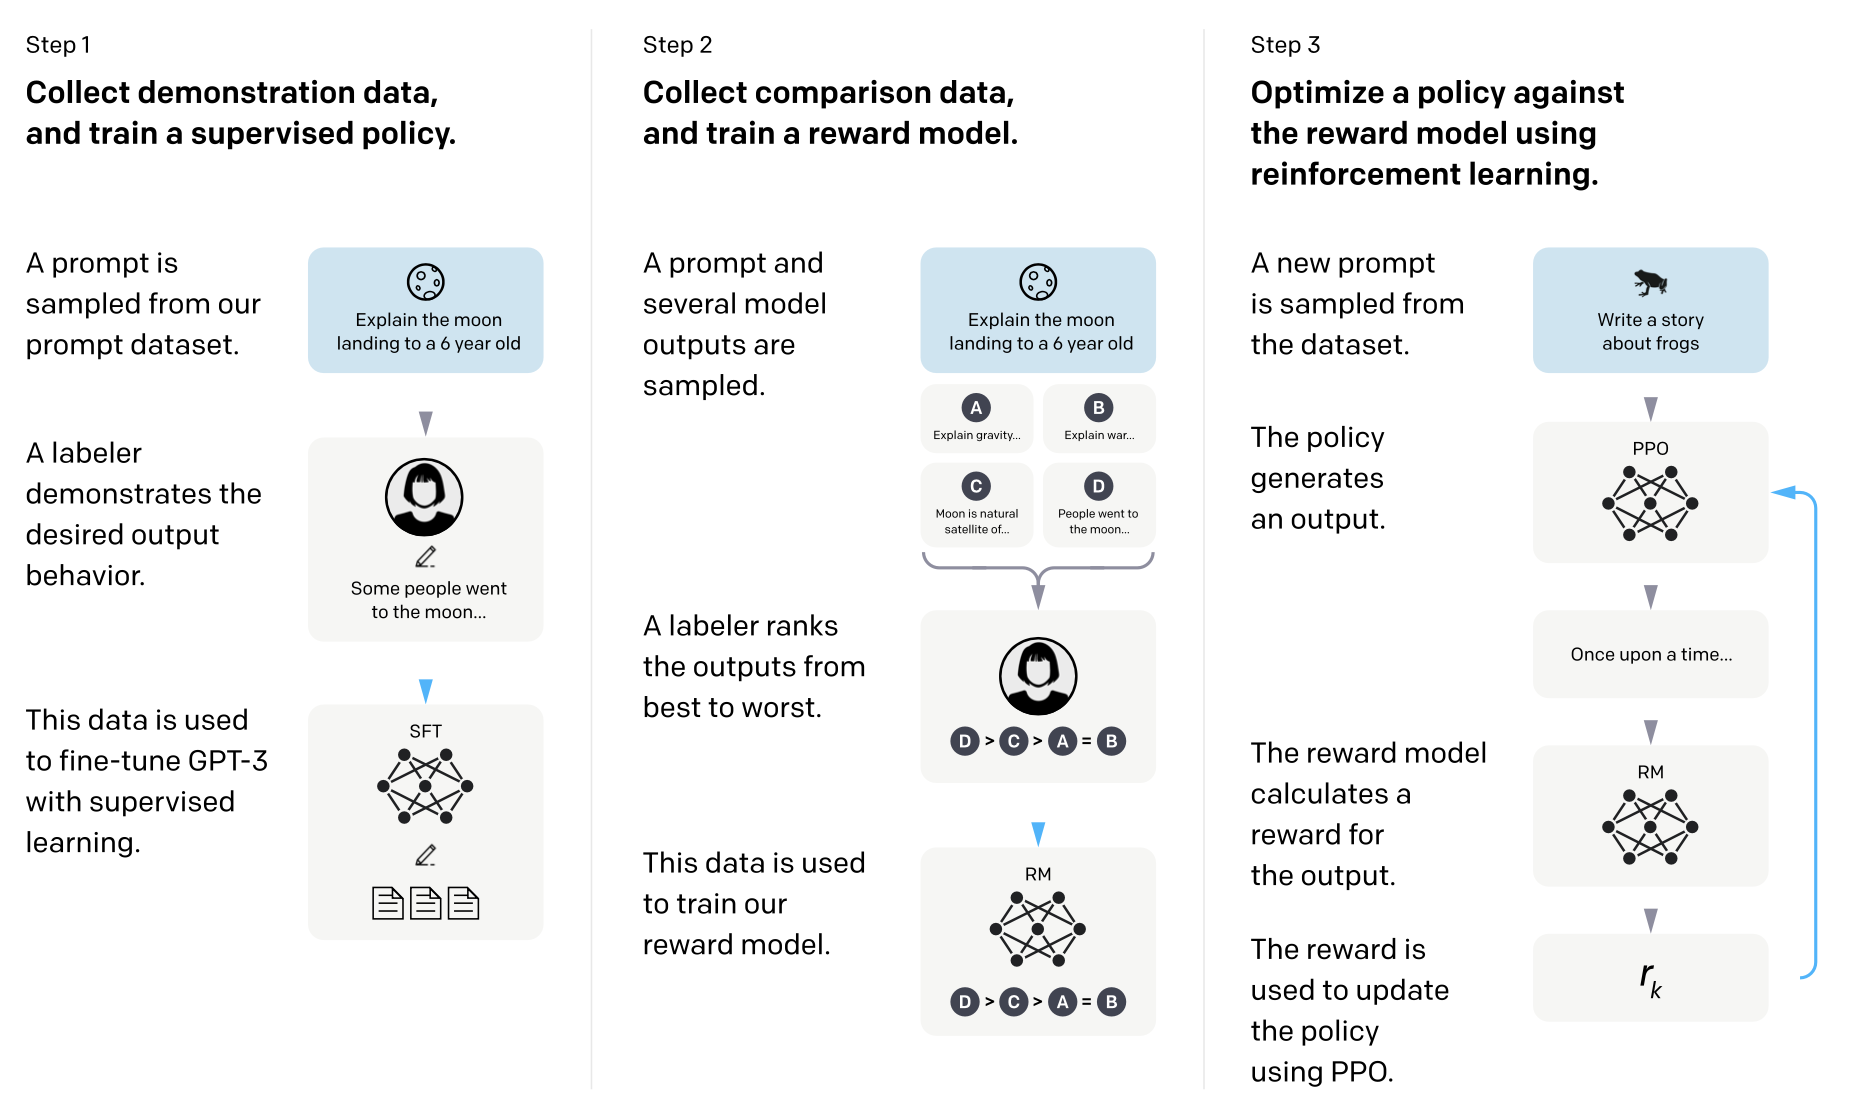
\includegraphics[width=0.9\linewidth]{./fig/rlhf_fig2.png}
  \caption{RLHFのプロセス\cite{InstructGPT}}
  \label{fig:rlhf_process}
\end{figure*}

\begin{enumerate}
  \item \textbf{教師ありファインチューニング (SFT):}
  高品質な指示応答データセットで事前学習済みモデルをファインチューニングし、後の強化学習の初期ポリシー(方策)$\pi^{\text{SFT}}$を形成する。

  \item \textbf{報酬モデルの学習:}
  SFTモデルに複数の応答を生成させ、人間がその好ましさをランク付けする。この選好データを用いて、応答の良し悪しを予測する報酬モデル$r_{\theta}$を学習させる。

  \item \textbf{強化学習による最適化:}
  報酬モデルを報酬関数とし、強化学習アルゴリズム(PPOなど)を用いて、報酬が最大化されるようにSFTモデルのパラメータを更新する。具体的には、以下の目的関数を最大化するように方策$\pi_{\phi}^{\text{RL}}$を最適化する\cite{InstructGPT}。
  $$
  \text{objective}(\phi) = \mathbb{E}_{(x,y) \sim D_{\pi_{\phi}^{\text{RL}}}} [r_{\theta}(x, y) - \beta \log(\pi_{\phi}^{\text{RL}}(y|x) / \pi^{\text{SFT}}(y|x))]
  $$
  ここで、第一項の$r_{\theta}(x, y)$は報酬モデルからの報酬を表す。第二項の$\log(\pi_{\phi}^{\text{RL}}(y|x) / \pi^{\text{SFT}}(y|x))$は、強化学習によって更新される方策$\pi_{\phi}^{\text{RL}}$と、元のSFTモデルの方策$\pi^{\text{SFT}}$との間のKLダイバージェンスの推定値であり、これが「\textbf{KLペナルティ}」として機能する。このペナルティ項(係数$\beta$で強度を調整)により、モデルが報酬モデルの欠陥を突いて質の低い出力を生成する「報酬ハッキング」を防ぎつつ、事前学習で獲得した言語能力が大きく損なわれることを抑制する効果がある。
\end{enumerate}
このRLHFの導入により、モデルの出力はより安全で、有用で、人間の意図に沿ったものになる。









\chapter{機械読解データセット}
\label{chap:datasets}
本研究は、既存の高品質なデータセットを転用して、新たな評価データセットを自動生成するアプローチを取る。本章では、その基盤となる機械読解データセットSQuADと、本研究で中核的に利用するその日本語版JSQuADについて詳述する。

\section{SQuAD (Stanford Question Answering Dataset)}

SQuADは、Rajpurkarらによって提案された\cite{SQuAD}、機械読解の研究を推進するための大規模データセットである。その登場以降、質問応答システムの性能を測るための事実上の標準ベンチマークとして、この分野の研究に絶大な影響を与えてきた。SQuADの最大の特徴は、その質問応答ペアがクラウドソーシングを通じて人間によって生成されている点にある。具体的には、Wikipediaの記事を文脈とし、クラウドワーカーがその内容に関する質問と、回答となる箇所を文脈中から連続した一部分(スパン)として抜き出すことで、10万件を超えるデータセットを構築している。この「\textbf{extractive question answering}」と呼ばれる形式は、モデルが回答を自由に生成するのではなく、文脈中のどこに答えが書かれているかを正確に特定する能力を求めるものであり、客観的な評価を可能にした。評価には、予測と正解が完全に一致するかを見るExact Match (EM)と、単語単位の一致度を測るF1 Scoreが用いられる\cite{SQuAD}。

\section{JSQuAD (Japanese Question Answering Dataset)}

JSQuADは、日本語の汎用言語理解ベンチマークJGLUE\cite{JGLUE}の一部として、Kuriharaらによって構築された、日本語の読解能力を評価するための大規模データセットである。その設計思想と構築プロセスは、SQuAD\cite{SQuAD}を基礎としており、日本語版Wikipediaの記事をソースに、クラウドソーシングによって約7万件の質問応答ペアが作成されている。図\ref{fig:jsquad_example}にそのデータ構造例を示す。

%% 画像ファイル "jsquad.jpg" を "fig" フォルダ内に配置してください
\begin{figure*}[t]
  \centering
  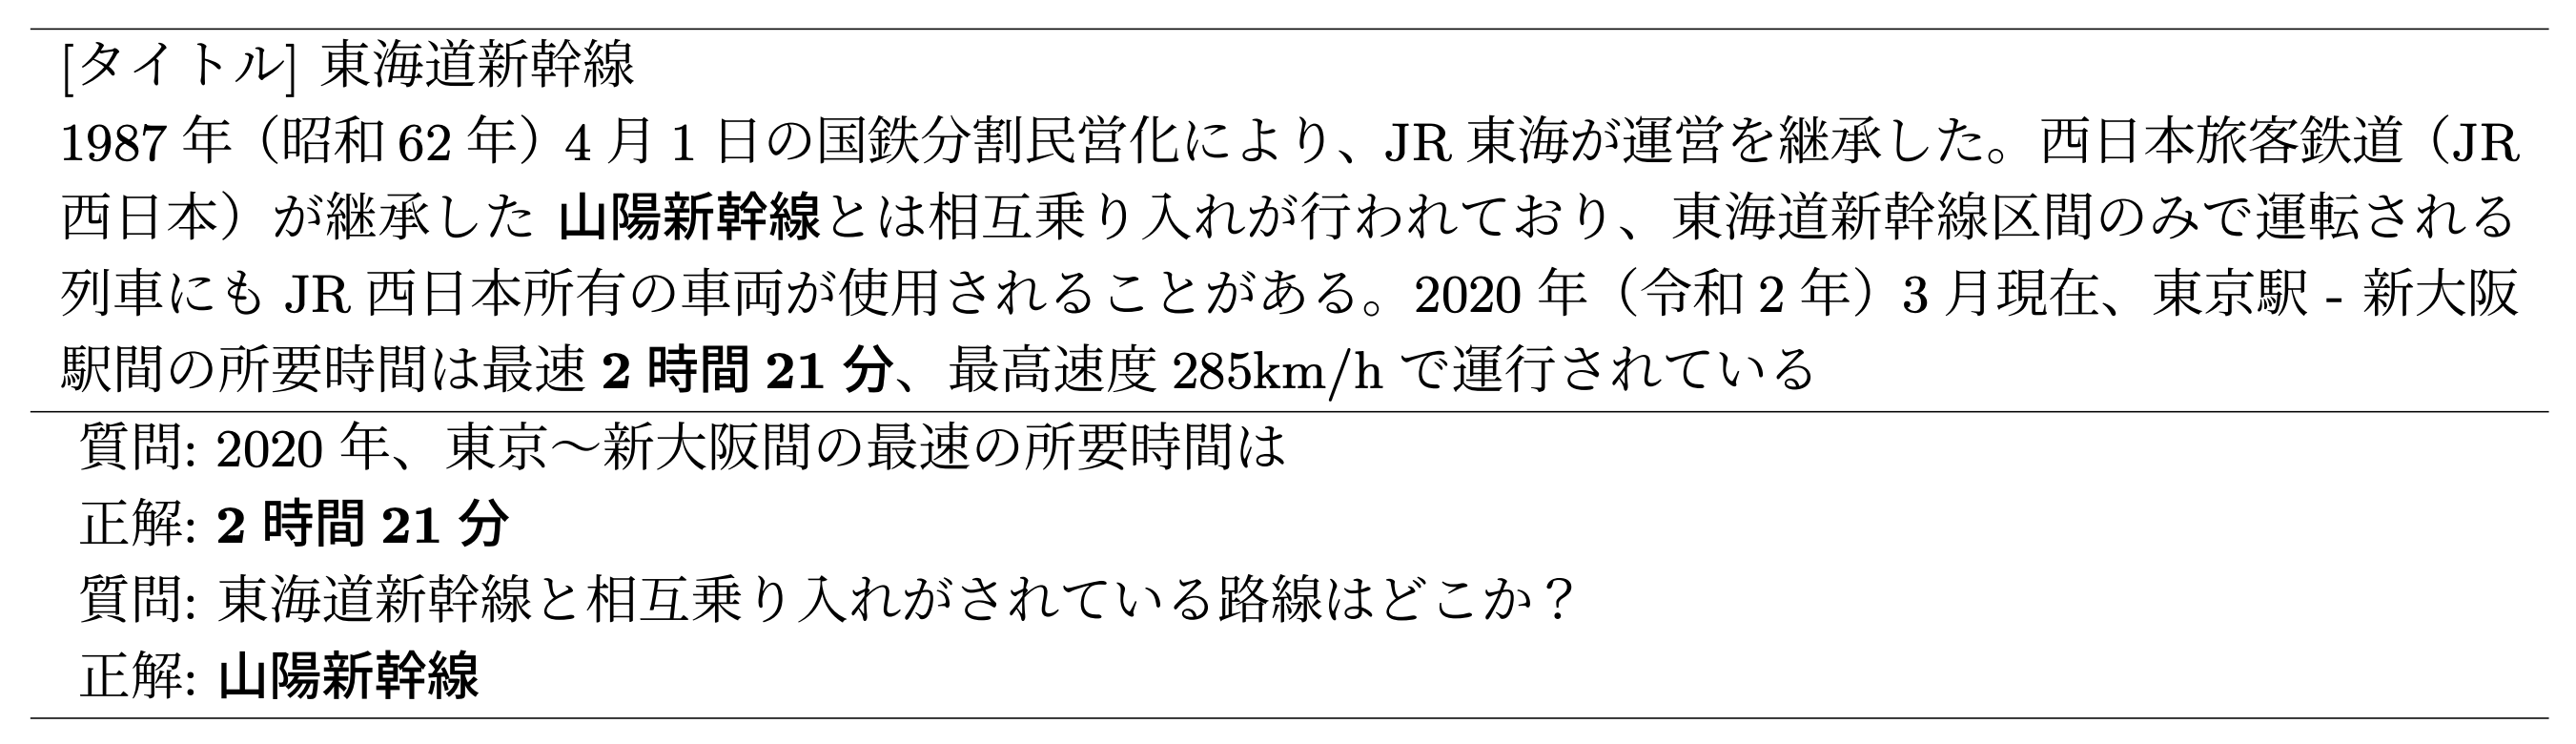
\includegraphics[width=0.9\linewidth]{./fig/jsquad.png}
  \caption{JSQuADのデータ構造例\cite{JGLUE}}
  \label{fig:jsquad_example}
\end{figure*}

評価指標もSQuADと同様にEMとF1スコアが採用されているが、日本語の特性を考慮した重要な工夫がなされている。日本語は単語の区切りが自明ではないため、分かち書きに用いる形態素解析器によって評価値が変動しうる。この問題を回避するため、JSQuADにおけるF1スコアは\textbf{文字単位(character-level)}で計算される\cite{JGLUE}。これにより、形態素解析器の違いに依存しない、安定した評価を実現している。

本研究では、このJSQuADを2つの重要な役割で活用する。第一に、次章で詳述する通り、その高品質なデータ構造を転用してQAペア生成モデルを学習させる「教師」として。第二に、実験の章において、自動生成された評価データセットの有効性を評価するための「審判」、すなわち人間が作成した基準(ゴールドスタンダード)としてである。





\chapter{関連研究}
\label{chap:related_work}

本研究は、既存の高品質なデータセットを転用して、新たな評価データセットを自動生成するアプローチを取る。本章では、LLMによるデータ生成に関する主要な先行研究として、Self-Instructと指示事前学習(Instruction Pre-Training)を取り上げ、本研究の位置づけを明確にする。

\section{Self-Instruct}

Self-Instructは、Wangらによって提案された\cite{Self-Instruct}、大規模言語モデル(LLM)自身を用いて、そのモデルの指示追従能力を向上させるための大規模な指示データセットを生成するフレームワークである。このアプローチは、人間による大規模なアノテーションコストをかけずに、既存の事前学習済みLLMの能力を最大限に引き出すことを目的としている。

そのプロセスは、図\ref{fig:self_instruct_example}に示すように、まず人間が作成した少数の多様な指示(論文では175個)を「シードセット」として用いることから始まる。このシードセットを基に、LLM(論文ではGPT-3)に対して自己生成的なプロンプティングを行い、新たな指示を生成させる。次に、生成された新しい指示が、既存の指示と類似しすぎていないか、あるいは不適切な内容でないかをフィルタリングする。そして、フィルタリングを通過した質の高い新規指示に対して、再度LLMを用いて、その指示を解くための具体的なインスタンス(入力と出力のペア)を生成させる。この一連の「指示生成→フィルタリング→インスタンス生成」のパイプラインを繰り返すことで、指示データセットを自己増殖的に拡張していく。

%% 画像ファイル "self-instruct_fig1.jpg" を "fig" フォルダ内に配置してください
\begin{figure*}[t]
  \centering
  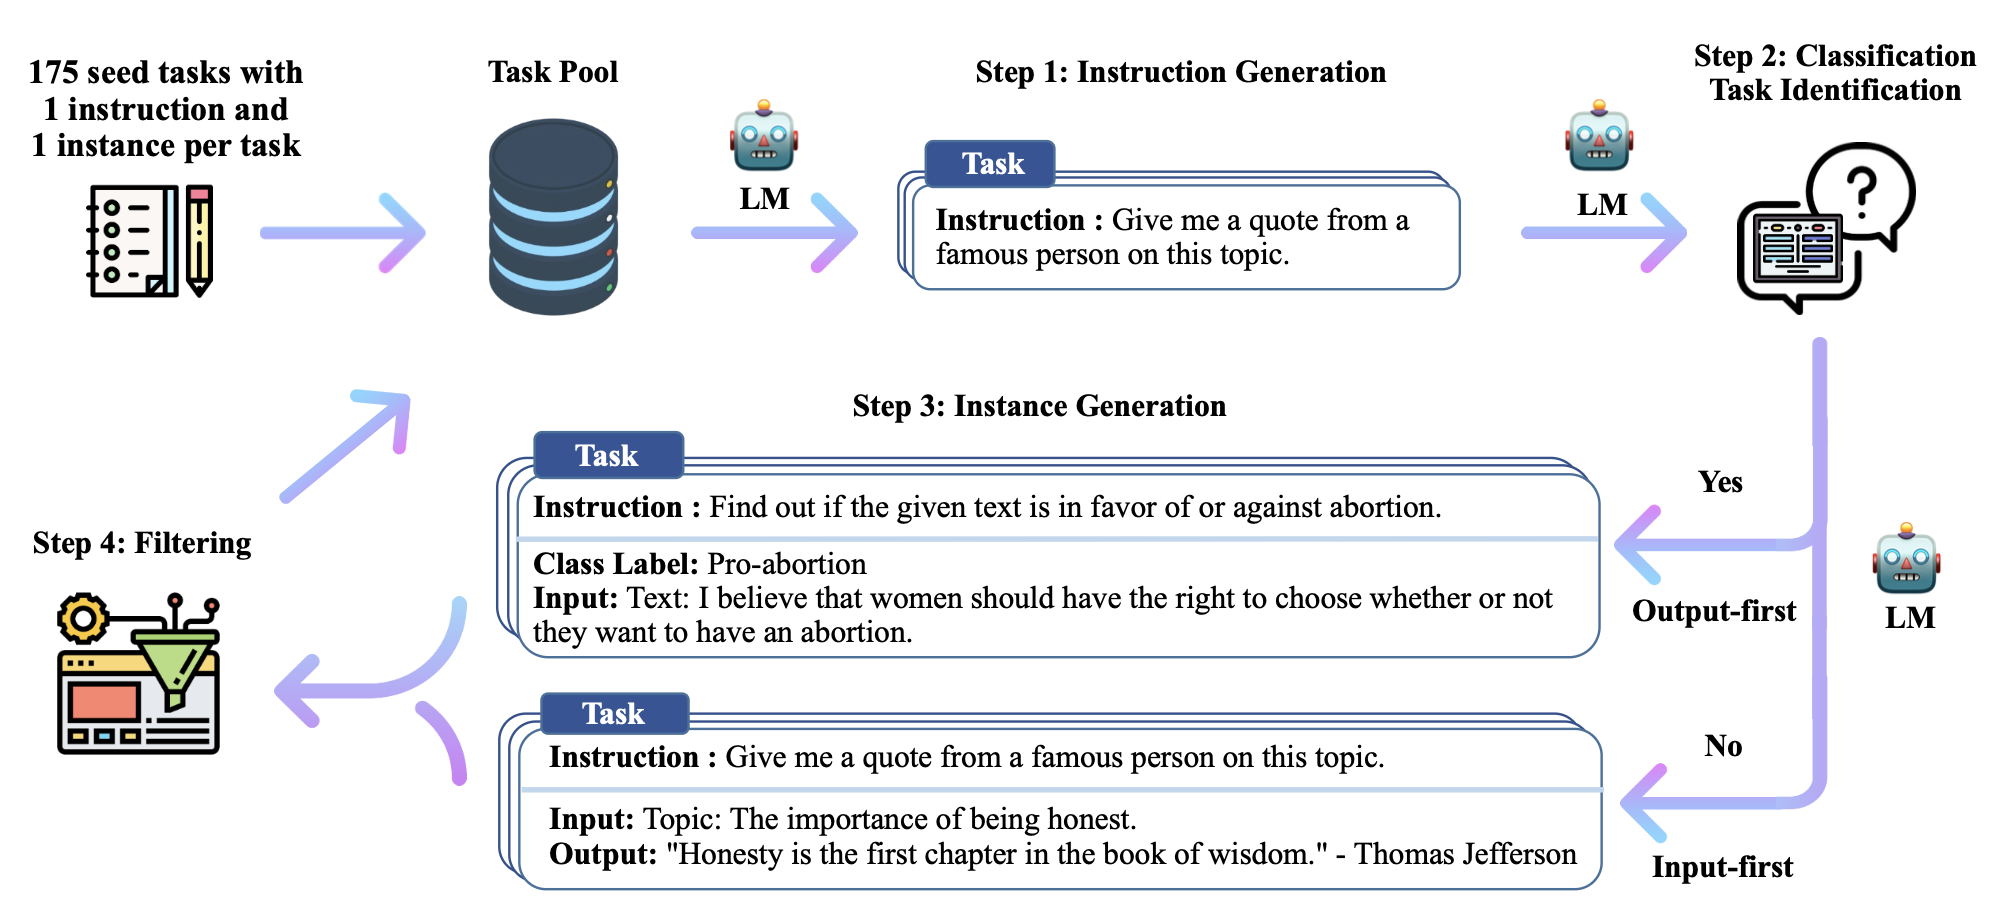
\includegraphics[width=0.9\linewidth]{./fig/self-instruct_fig1.png}
  \caption{Self-Instructのデータ生成パイプライン\cite{Self-Instruct}}
  \label{fig:self_instruct_example}
\end{figure*}

この研究の重要な貢献は、このようにして自動生成されたデータセット(論文では52,000件以上)で、元の事前学習済みLLMをファインチューニングすることにより、その指示追従能力が大幅に向上することを示した点にある。実際、ファインチューニング後のモデルは、元のGPT-3の性能を上回り、人間による評価では当時最高性能であった`text-davinci-001`に匹敵する結果を示した\cite{Self-Instruct}。

本研究のアプローチは、LLMを用いて学習データを合成するという点でSelf-Instructと共通している。しかし、両者には明確な差異が存在する。Self-Instructが少数のシードから多様なタスクの指示をゼロから生成し、モデルの汎用的な指示追従能力の向上を目指すのに対し、本研究は既存の高品質な読解データセット(JSQuAD)のデータ構造を転用し、特定の目的(評価データ生成)に特化したデータを生成する。特に、本研究のアプローチは、常に信頼できる「文脈」に事実を基づかせることで、Self-Instructで課題となりうるハルシネーションを原理的に抑制する設計となっている点が異なる。

\section{指示事前学習 (Instruction Pre-Training)}

指示事前学習(Instruction Pre-Training)は、Chengらによって提案された\cite{Instruction Pre-Training}、言語モデルの事前学習段階そのものに、教師ありの指示データを大規模に組み込む新しいフレームワークである。従来、LLMの事前学習はラベルなしの生コーパスのみを用いる自己教師あり学習(Vanilla Pre-Training)が主流であったが、本手法では事前学習の段階からモデルに多様なタスクを解く能力を学習させることを目的とする。

そのプロセスは、図\ref{fig:instruction_pretraining_example}に示すように、まず「指示シンセサイザ(instruction synthesizer)」と呼ばれるモデルを用いて、生コーパスの内容に基づいた「指示と応答(instruction-response)」のペアを大量に自動生成する。次に、元の生コーパスと生成された指示応答ペアを組み合わせた「指示拡張コーパス(instruction-augmented corpora)」を構築し、これを最終的な事前学習データとして用いる。このアプローチの核心は、生コーパスの内容に事実を基づかせた(Fact-Grounded)教師あり信号を、事前学習の段階でモデルに与える点にある。

%% 画像ファイル "instruction-pretraining_fig1.png" を "fig" フォルダ内に配置してください
\begin{figure*}[t]
  \centering
  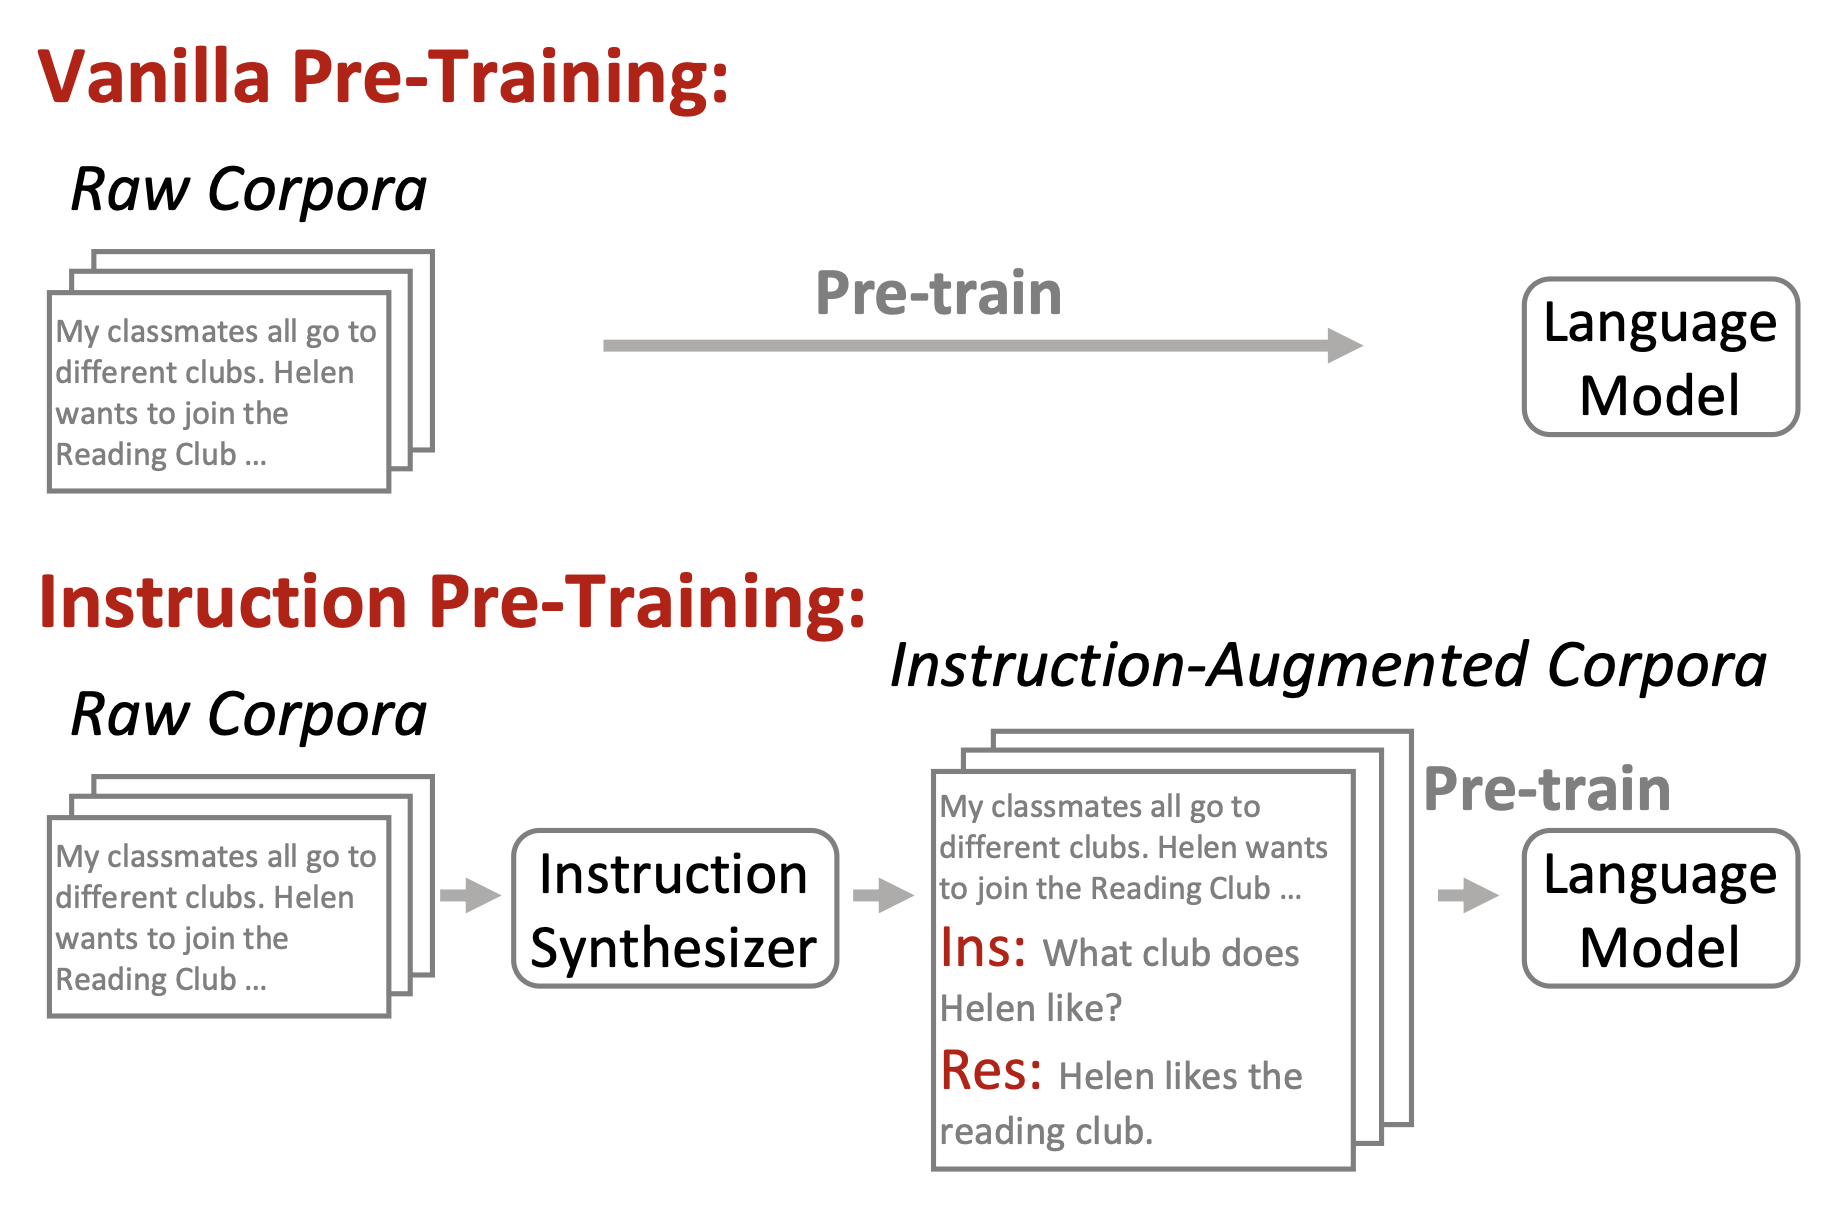
\includegraphics[width=0.9\linewidth]{./fig/instruction-pretraining_fig1.png}
  \caption{一般的な事前学習と指示事前学習の違い\cite{Instruction Pre-Training}}
  \label{fig:instruction_pretraining_example}
\end{figure*}

この指示シンセサイザは、SQuADやHotpotQAなど多様な既存データセットを「文脈から指示と応答のペアを生成する」という形式に変換して学習データとし、オープンソースの言語モデル(例:Mistral-7B)をファインチューニングすることで構築される\cite{Instruction Pre-Training}。このアプローチは、本研究における「JSQuADのデータ構造を組み替えて指示チューニングデータを作成する」という着想と非常に親和性が高い。しかし、本論文がモデルの汎用的な能力向上を目指して事前学習の段階で指示データを導入するのに対し、本研究では評価用データセットの生成という特定の目的のためにファインチューニング段階で指示チューニングを活用する点で、目的と適用段階が明確に異なる。

論文では、この手法で事前学習されたモデルは、従来のモデルを上回る性能を示すだけでなく、その後の指示チューニングからもより大きな恩恵を受けることが示されている\cite{Instruction Pre-Training}。これは、事前学習とファインチューニングのタスク形式が近接することで、両段階の移行がよりスムーズになるためだと考察されており、本研究のアプローチの有効性を間接的に支持する知見と言える。








\chapter{提案手法}
\label{chap:proposal}
本章では、信頼性の高い日本語評価データを自動生成するための提案手法について詳述する。本手法は、評価データを生成する「生成アプローチ」と、その有効性を検証するための「テストフレームワーク」の2つの主要な要素から構成される。

\section{評価データ生成アプローチ}
本研究では、提案手法の有効性を多角的に示すため、異なるアプローチで評価データを生成し、その結果を比較する。生成モデルには、東京科学大学が公開しているLlama-3.1-Swallow-8B-Instruct-v0.3\cite{Fujii:COLM2024}を一貫して使用する。理由としては、大規模な日本語コーパスで継続事前学習されており、日本語データセットによる指示チューニングも行われているため、日本語の指示に対する応答生成能力が高いことが挙げられる。生成に使用したプロンプトは付録\ref{chap:appendix_b}に示す。

\subsection{ベースライン手法}
提案手法の優位性を際立たせるためには、より単純な手法との比較が不可欠である。本研究では、追加の学習を行わない「Zero-Shot推論」と、少数の文脈内学習例を与える「Few-Shot推論」をベースラインとして設定する。

\subsubsection{Zero-Shot推論(ベースライン1)}
Zero-Shot推論は、追加の学習や具体例の提示なしに、一般的な指示のみでタスクを遂行させる最も基本的なアプローチである。これは、LLMが持つ汎用的な指示理解能力と文脈読解能力のみに依存する方法であり、本実験における性能の下限を測るためのベースラインとして機能する。具体的には、「この文章に基づいて質問と回答を生成してください」といった指示プロンプトと文脈情報を生成モデルに与え、QAペアの評価データを生成させる。

\subsubsection{10-Shot推論(ベースライン2)}
10-Shot推論は、プロンプト内に少数のQA生成の模範例を提示し、モデルの文脈内学習(in-context learning)能力を評価するアプローチである。モデルは提示された例のパターンを即座に学習し、タスクをより正確に遂行することが期待される。本研究では、JSQuADの学習データから抽出した10個の「文脈、質問、回答」のペアを例としてプロンプトに含めることで、Zero-Shot推論からの性能向上を検証する。

\subsection{指示チューニングによる生成(提案手法)}
本研究の主軸となるアプローチが、指示チューニング\cite{Instruction-Tuning}の活用である。この手法の独創的な核心は、高品質な読解データセットであるJSQuAD\cite{JSQuAD}を、QAペア生成モデルの学習用途として効果的に活用する点にある。

本来、JSQuADは図\ref{fig:repurposing_jsquad}の上段に示すように、「文脈」と「質問」を入力とし、「回答」を予測する読解タスク用に設計されている。本研究ではこの入出力構造を意図的に組み替え、図\ref{fig:repurposing_jsquad}の下段のように「文脈」のみを入力とし、対応する「質問と回答のペア」全体を出力するようにタスクを再定義した。この発想の転換により、読解モデル評価用のデータセットを、QAペア生成モデルの学習用教師データとして活用することが可能となる。これにより、モデルは文脈から適切な問いと答えを創出するという、より専門的な能力を直接的に学習する。学習後には、未知の文脈を入力するだけで、その内容に基づいた高品質なQA形式の評価データを生成できるようになる。

%% 画像ファイル "proposal_fig1.png" を "fig" フォルダ内に配置してください
\begin{figure*}[t]
  \centering
  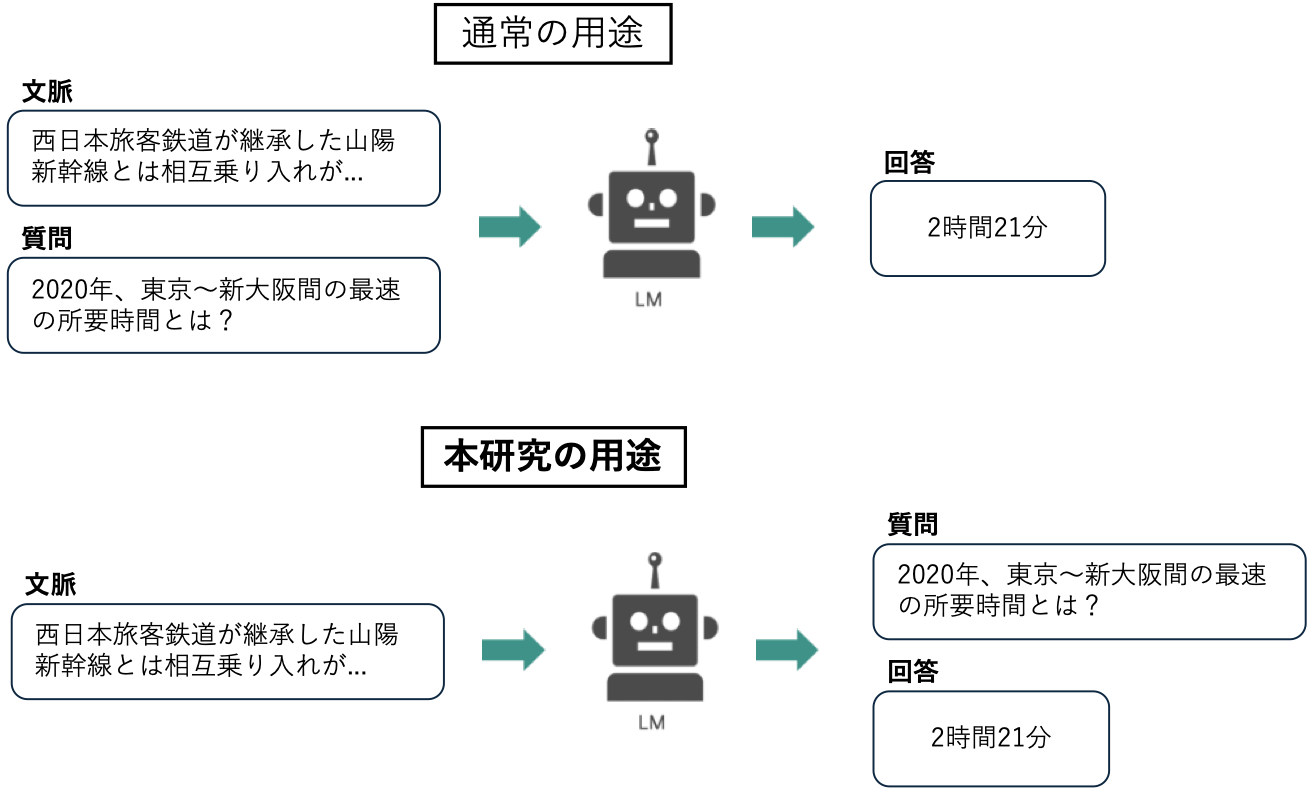
\includegraphics[width=\linewidth]{./fig/proposal_fig1.png}
  \caption{JSQuADのデータ構造の組み替えによる生成モデルの学習}
  \label{fig:repurposing_jsquad}
\end{figure*}

\section{有効性評価のためのテストフレームワーク}
上記のアプローチで生成した各評価データセットの有効性をテストするため、統一されたテストフレームワークを構築した。性能評価の基準(ベースライン)として、人間が作成したJSQuADの検証データセットを本来の読解タスクとして用いる。これは、人間が作成した評価データがLLMの評価には最適という前提に基づいている。この基準データセットを、表\ref{tab:target_llms}に示す12種類のオープンソースLLM群に解かせ、それぞれの正解率(回答の完全一致率)を基に「モデル性能の基準ランキング」を算出する。次に、自動生成した各評価データセットを用いて同様に12モデルの性能ランキングをそれぞれ算出する。最終的に、「基準ランキング」と「自動生成データによるランキング」との間にどの程度の相関があるかを、スピアマンの順位相関係数($\rho$)を用いて定量的に評価する。この$\rho$値が1に近いほど、自動生成された評価データが、人手によるベンチマークと同等の信頼性を持つ評価軸として機能することを示す。

\begin{table*}[t]
  \centering
  \caption{評価対象としたオープンソースLLM(12種類)}
  \label{tab:target_llms}
  \begin{tabular}{|l|l|}
    \hline
    gemma-2-9b-it & aya-23-8B \\
    Qwen2.5-7B-Instruct & gemma-2-2b-it \\
    gemma-2-2b-jpn-it & Qwen2.5-14B-Instruct \\
    Meta-Llama-3.1-8B-Instruct & aya-expanse-8b \\
    Qwen2.5-3B-Instruct & Ministral-8B-Instruct-2410 \\
    Meta-Llama-3-8B-Instruct & Mistral-7B-Instruct-v0.3 \\
    \hline
  \end{tabular}
\end{table*}


\chapter{実験}

\section{目的}
本実験の目的は、3章で述べた提案手法の有効性を実証することにある。具体的には、3つの生成アプローチ(Zero-Shot推論、10-Shot推論、指示チューニング)で作成した評価データが、人間製ベンチマーク(JSQuAD)によるLLMの性能ランキングをどの程度忠実に再現できるかを、スピアマンの順位相関係数を用いて定量的に比較・評価する。

\section{実験設定}
実験の主要な設定は表\ref{tab:exp_setting_main}に示す通りである。評価対象には、表\ref{tab:target_llms}にリストアップした12種類のオープンソースLLMを選定し、推論用に4bit量子化されたgguf形式に変換して使用した。

\begin{table}[h]
  \centering
  \caption{主要な実験設定}
  \label{tab:exp_setting_main}
  \begin{tabularx}{0.9\linewidth}{lX}
  \hline
  項目       & 内容 \\
  \hline
  生成モデル   & `tokyotech-llm/Llama-3.1-Swallow-8B-Instruct-v0.3` \\
  学習データ   & JSQuAD (日本語版SQuAD) \\
  比較手法   & Zero-Shot推論、10-Shot推論 \\
  評価対象モデル & 表\ref{tab:target_llms}記載の12種類 (4bit量子化) \\
  基準データ   & JSQuAD検証データセット \\
  評価指標     & スピアマンの順位相関係数 ($\rho$) \\
  \hline
  \end{tabularx}
\end{table}

\section{実験結果}
\subsection{基準ランキング(人間製データによるテスト)}
まず、有効性評価の基準となる、人間が作成したJSQuADデータセットにおける12モデルの性能ランキングを算出した。結果を表\ref{tab:baseline_ranking}に示す。このランキングが、本実験において再現を目指す「正解」の序列となる。

\begin{table}[h]
  \centering
  \caption{基準ランキング(JSQuADデータによるテスト結果)}
  \label{tab:baseline_ranking}
  \begin{tabular}{clc}
    \hline
    Rank & Model Name & Accuracy (\%) \\
    \hline
    1 & gemma-2-9b-it & 55.02 \\
    2 & aya-23-8B & 54.59 \\
    3 & Qwen2.5-7B-Instruct & 46.04 \\
    4 & gemma-2-2b-it & 44.57 \\
    5 & gemma-2-2b-jpn-it & 43.76 \\
    6 & Qwen2.5-14B-Instruct & 43.43 \\
    7 & Meta-Llama-3.1-8B-Instruct & 40.18 \\
    8 & aya-expanse-8b & 40.12 \\
    9 & Qwen2.5-3B-Instruct & 35.86 \\
    10 & Ministral-8B-Instruct-2410 & 33.14 \\
    11 & Meta-Llama-3-8B-Instruct & 28.12 \\
    12 & Mistral-7B-Instruct-v0.3 & 0.41 \\
    \hline
  \end{tabular}
\end{table}

\subsection{各生成アプローチによる評価データのテスト結果}
次に、3つのアプローチで生成した評価データを用いて、それぞれ同様のテストを行った。各手法における性能ランキングと、基準ランキングとのスピアマンの順位相関係数を表\ref{tab:results_summary}にまとめる。詳細なランキングは\ref{chap:appendix_a}に示す。

\begin{table}[h]
  \centering
  \caption{各生成アプローチと基準ランキングとの順位相関係数}
  \label{tab:results_summary}
  \begin{tabular}{lc}
  \hline
  生成アプローチ       & 順位相関係数 ($\rho$) \\
  \hline
  Zero-Shot 推論       & 0.6364 \\
  10-Shot 推論         & 0.7622 \\
  指示チューニング(提案手法) & \textbf{0.8741} \\
  \hline
  \end{tabular}
\end{table}

\section{考察}
表\ref{tab:results_summary}が示す通り、相関係数はZero-Shot推論の$\rho=0.6364$から、10-Shot推論で$\rho=0.7622$へ、そして指示チューニングでは$\rho=0.8741$へと段階的に向上した。この傾向は、生成モデルへの指示をより具体的に、かつタスクに特化させるほど、生成される評価データの信頼性が向上することを示唆している。

特に、本研究の主軸である指示チューニングアプローチが高い相関を達成したことは、JSQuADのデータ構造を組み替えて学習させるという本手法の有効性を強く裏付けている。これにより、人間が作成したベンチマークの評価軸を忠実に再現可能であることが実証された。

なお、自動生成された評価データを用いた際の各モデルの絶対的な正解率は、人間製データを用いた際よりも全体的に低下する傾向が見られた。これは生成された問題の難易度や表現の揺れに起因すると考えられる。しかし、評価データセットとしての最も重要な役割である、モデル間の相対的な性能差を正確に捉え、信頼性の高い性能ランキングを構築するという点において、本提案手法は十分に有効であることが、この高い順位相関係数によって示されている。






\chapter{結論}
\section{まとめ}
本研究は、日本語LLMの評価データセット不足という課題に対し、LLMを用いて信頼性の高いテストデータを低コストかつスケーラブルに自動生成する手法を提案した。提案手法の核心は、ハルシネーションを抑制するために信頼できる「文脈」に事実を基づかせ、高品質な人間製データセットJSQuADのデータ構造を転用して生成モデルを「指示チューニング」する点にある。

実験を通じて、提案手法である指示チューニングが、Zero-ShotやFew-Shotといったベースライン手法を大幅に上回り、人間製ベンチマークと極めて高い性能相関($\rho = 0.8741$)を持つことを実証した。この結果は、「文脈情報に基づいてテストデータを自動生成する」という本研究のアプローチ全体の有効性を示すものである。本研究の成果は、不足している日本語評価基盤の構築を促進し、今後の日本語LLMの研究開発エコシステムの発展に貢献することが期待される。

\section{今後の課題}
本研究の成果を基盤とし、将来的には以下のような方向性で研究を発展させることを目指す。

第一に、Reasoning LLMの活用可能性の探求である。予備実験において、学習なしのReasoning LLMがZero-Shot推論で極めて高い性能($\rho = 0.9580$)を示すことが確認された。この現象の背景にあるメカニズムの解明や、専門的な指示チューニングモデルとの性能差が生まれる要因を深く分析することは、今後の重要な研究課題である。

第二に、強化学習による品質向上である。予備実験では、GRPOを用いた強化学習が、ランキング再現性($\rho$)と問題の質(絶対正解率)の間でトレードオフを生む可能性が示唆された。今後は報酬関数の設計を洗練させ、これらの指標を両立させるアプローチを探求する。

第三に、異言語・特定ドメインへの展開である。予備実験では、英語データセットSQuADで学習したモデルを日本語生成に単純適用することの困難さが示された。英語の豊富なデータ資産を、日本語やその他の低リソース言語、あるいは特定の専門ドメイン(医療、法律など)の評価データ生成に効果的に活用するための、より高度な言語転移技術の開発が望まれる。

最後に、テストフォーマットの拡張である。現在の一問一答形式に加え、複数選択肢形式や、より複雑な推論を要するマルチホップ質問応答形式のテストデータを自動生成する手法の開発に取り組む。

\chapter*{謝辞}
\addcontentsline{toc}{chapter}{\numberline{}謝辞}
本研究を進めるにあたり、指導教員である筑波大学システム情報系情報工学域山本幹雄教授、
筑波大学システム情報系情報工学域乾孝司准教授、
筑波大学システム情報系情報工学域津川翔准教授からは非常に多くの助言を頂きました。
心より感謝申し上げます。
特に、常日頃から研究活動や論文執筆において大変多くのご指導を頂きました山本幹雄教授に深く感謝申し上げます。
また、論文を書き上げるにあたってさまざまサポートをしていただいた研究室の皆様に感謝申し上げます。

\newpage
\addcontentsline{toc}{chapter}{\numberline{}参考文献}
\renewcommand{\bibname}{参考文献}

\begin{thebibliography}{99}
  \bibitem{Instruction-Tuning}
  Jason Wei, Maarten Bosma, Vincent Y. Zhao, Kelvin Guu, Adams Wei Yu, Brian Lester, Nan Du, Andrew M. Dai, Quoc V. Le. Finetuned Language Models Are Zero-Shot Learners. arXiv:2109.01652. 2021.
  \bibitem{Instruction Pre-Training}
  Daixuan Cheng, Yuxian Gu, Shaohan Huang, Junyu Bi, Minlie Huang, Furu Wei. Instruction Pre-Training: Language Models are Supervised Multitask Learners. arXiv:2406.14491. 2024.
  \bibitem{SQuAD}
  Pranav Rajpurkar, Jian Zhang, Konstantin Lopyrev, Percy Liang. SQuAD: 100,000+ Questions for Machine Comprehension of Text. arXiv:1606.05250. 2016.
  \bibitem{JSQuAD}
  Soichi Yasunaga, Juro Fukunaga, et al. JSQuAD: A Japanese Question Answering Dataset. arXiv:2202.01764. 2022.
  \bibitem{JGLUE}
  Kurihara Kentaro, Kawahara Daisuke, Shibata Tomohide. JGLUE: Japanese General Language Understanding Evaluation. https://aclanthology.org/2022.lrec-1.317. 2022.
  \bibitem{Fujii:COLM2024}
  Kazuki Fujii, Taishi Nakamura, Mengsay Loem, Hiroki Iida, Masanari Ohi, Kakeru Hattori, Hirai Shota, Sakae Mizuki, Rio Yokota, Naoaki Okazaki. Continual Pre-Training for Cross-Lingual LLM Adaptation: Enhancing Japanese Language Capabilities. Proceedings of the First Conference on Language Modeling. 2024.
  \bibitem{Okazaki:COLM2024}
  Naoaki Okazaki, Kakeru Hattori, Hirai Shota, Hiroki Iida, Masanari Ohi, Kazuki Fujii, Taishi Nakamura, Mengsay Loem, Rio Yokota, Sakae Mizuki. Building a Large Japanese Web Corpus for Large Language Models. Proceedings of the First Conference on Language Modeling. 2024.
  \bibitem{ma:arxiv2025}
  Youmi Ma, Sakae Mizuki, Kazuki Fujii, Taishi Nakamura, Masanari Ohi, Hinari Shimada, Taihei Shiotani, Koshiro Saito, Koki Maeda, Kakeru Hattori, Takumi Okamoto, Shigeki Ishida, Rio Yokota, Hiroya Takamura, Naoaki Okazaki. Building Instruction-Tuning Datasets from Human-Written Instructions with Open-Weight Large Language Models. arXiv:2503.23714. 2025.
  \bibitem{GPT-3}
  Tom B. Brown, Benjamin Mann, Nick Ryder, Melanie Subbiah, Jared Kaplan, Prafulla Dhariwal, et al. Language Models are Few-Shot Learners. arXiv:2005.14165. 2020.
\end{thebibliography}










\chapter*{付録A 各生成アプローチの詳細な実験結果}
\addcontentsline{toc}{chapter}{\numberline{}付録A 各生成アプローチの詳細な実験結果}
\label{chap:appendix_a}

本章では、第4章で述べた実験における、各生成アプローチで得られた評価対象モデルの性能ランキングの詳細を示す。

\section{Zero-Shot推論による評価結果}
\begin{table}[hbtp]
  \centering
  \caption{Zero-Shot推論で生成したデータセットによる評価結果}
  \label{tab:appendix_zero_shot}
  \begin{tabular}{clcc}
    \hline
    Rank & Model Name & Accuracy (\%) & Score (Correct/Total) \\
    \hline
    1 & aya-23-8B & 7.09 & 315/4442 \\
    2 & Ministral-8B-Instruct-2410 & 6.64 & 295/4442 \\
    3 & gemma-2-9b-it & 6.64 & 295/4442 \\
    4 & Qwen2.5-7B-Instruct & 6.26 & 278/4442 \\
    5 & gemma-2-2b-jpn-it & 6.06 & 269/4442 \\
    6 & Qwen2.5-14B-Instruct & 5.97 & 265/4442 \\
    7 & Qwen2.5-3B-Instruct & 5.65 & 251/4442 \\
    8 & gemma-2-2b-it & 5.29 & 235/4442 \\
    9 & Meta-Llama-3.1-8B-Instruct & 4.91 & 218/4442 \\
    10 & Meta-Llama-3-8B-Instruct & 4.89 & 217/4442 \\
    11 & aya-expanse-8b & 4.19 & 186/4442 \\
    12 & Mistral-7B-Instruct-v0.3 & 0.74 & 33/4442 \\
    \hline
  \end{tabular}
\end{table}

\section{10-Shot推論による評価結果}
\begin{table}[hbtp]
  \centering
  \caption{10-Shot推論で生成したデータセットによる評価結果}
  \label{tab:appendix_10_shot}
  \begin{tabular}{clcc}
    \hline
    Rank & Model Name & Accuracy (\%) & Score (Correct/Total) \\
    \hline
    1 & gemma-2-9b-it & 7.54 & 335/4442 \\
    2 & Qwen2.5-7B-Instruct & 7.52 & 334/4442 \\
    3 & aya-23-8B & 7.34 & 326/4442 \\
    4 & Ministral-8B-Instruct-2410 & 7.32 & 325/4442 \\
    5 & gemma-2-2b-jpn-it & 6.66 & 296/4442 \\
    6 & Qwen2.5-14B-Instruct & 6.30 & 280/4442 \\
    7 & Meta-Llama-3.1-8B-Instruct & 6.26 & 278/4442 \\
    8 & Qwen2.5-3B-Instruct & 5.72 & 254/4442 \\
    9 & gemma-2-2b-it & 5.67 & 252/4442 \\
    10 & aya-expanse-8b & 4.91 & 218/4442 \\
    11 & Meta-Llama-3-8B-Instruct & 4.86 & 216/4442 \\
    12 & Mistral-7B-Instruct-v0.3 & 0.99 & 44/4442 \\
    \hline
  \end{tabular}
\end{table}

\section{指示チューニング(提案手法)による評価結果}
\begin{table}[hbtp]
  \centering
  \caption{指示チューニングで生成したデータセットによる評価結果}
  \label{tab:appendix_instruction_tuned}
  \begin{tabular}{clcc}
    \hline
    Rank & Model Name & Accuracy (\%) & Score (Correct/Total) \\
    \hline
    1 & gemma-2-9b-it & 18.91 & 840/4442 \\
    2 & aya-23-8B & 18.48 & 821/4442 \\
    3 & Qwen2.5-7B-Instruct & 16.28 & 723/4442 \\
    4 & Meta-Llama-3.1-8B-Instruct & 15.26 & 678/4442 \\
    5 & gemma-2-2b-jpn-it & 15.17 & 674/4442 \\
    6 & gemma-2-2b-it & 15.11 & 671/4442 \\
    7 & Ministral-8B-Instruct-2410 & 14.39 & 639/4442 \\
    8 & Qwen2.5-3B-Instruct & 13.28 & 590/4442 \\
    9 & Qwen2.5-14B-Instruct & 13.08 & 581/4442 \\
    10 & aya-expanse-8b & 13.01 & 578/4442 \\
    11 & Meta-Llama-3-8B-Instruct & 9.66 & 429/4442 \\
    12 & Mistral-7B-Instruct-v0.3 & 0.41 & 18/4442 \\
    \hline
  \end{tabular}
\end{table}








\chapter*{付録B 本研究で用いたプロンプト}
\addcontentsline{toc}{chapter}{\numberline{}付録B 本研究で用いたプロンプト}
\label{chap:appendix_b}

本章では、本研究における評価データの生成に用いたプロンプトのテンプレート、および指示チューニングの学習に用いたデータフォーマットを示す。

\section{推論時に使用したプロンプト}
評価データを生成する(推論)際に、各アプローチで用いたプロンプトは以下の通りである。

\subsection{Zero-Shot推論および指示チューニング済みモデル用}
Zero-Shot推論、および提案手法である指示チューニング済みモデルによる評価データ生成の際には、以下のプロンプトテンプレートを使用した。`{{ context }}`の部分には、JSQuADから抽出した文脈テキストが挿入される。

\begin{screen}
\begin{verbatim}
### 指示:
文脈から一問一答QAデータを一つだけ作成してください。

### 文脈:
{{ context }}

### 出力フォーマット:
次の形式で出力してください。
```json
{
  "question": "質問",
  "answer": "回答"
}
````

### 注意:

  - 質問は文脈に基づいていて、具体的かつ適切な内容にしてください。
  - 回答は文脈から直接導き出せる内容で、かつ簡潔にしてください。
  - 不適切または曖昧な質問や回答は避けてください。

### 応答:

\end{verbatim}
\end{screen}

\subsection{10-Shot推論用}
10-Shot推論の際には、事例(examples)を追加した以下のプロンプトテンプレートを使用した。`{{ examples }}`の部分にはJSQuADから抽出した10個のQAペアが、`{{ context }}`の部分には対象となる文脈テキストが挿入される。

\begin{screen}
\begin{verbatim}

### 指示:

事例を参考にして、文脈から一問一答QAデータを一つだけ作成してください。

### 事例:

{{ examples }}

### 文脈:

{{ context }}

### 出力フォーマット:

次の形式で出力してください。

```json
{
  "question": "質問",
  "answer": "回答"
}
```

### 注意:

  - 質問は文脈に基づいていて、具体的かつ適切な内容にしてください。
  - 回答は文脈から直接導き出せる内容で、かつ簡潔にしてください。
  - 不適切または曖昧な質問や回答は避けてください。

### 応答:

\end{verbatim}
\end{screen}

\section{指示チューニングの学習データに用いたフォーマット}
提案手法である指示チューニング済みモデルを学習させる際には、JSQuADのデータを以下の入力・出力フォーマットに変換して使用した。

\subsection{入力フォーマット}
学習時、モデルには以下の形式で入力が与えられる。`{{ context }}`の部分にはJSQuADの文脈テキストが入る。

\begin{screen}
\begin{verbatim}

### 指示:

文脈からQAデータを一つだけ作成してください。

### 文脈:

{{ context }}

### 出力フォーマット:

次の形式で出力してください。

```json
{
  "question": "質問",
  "answer": "回答"
}
```

### 注意:

  - 質問は文脈に基づいて具体的かつ適切な内容にしてください。
  - 回答は文脈から直接導き出せる内容にしてください。
  - 不適切または曖昧な質問や回答は避けてください。

### 応答:

\end{verbatim}
\end{screen}

\subsection{出力フォーマット}
モデルが学習すべき正解データ(出力)は、以下のJSON形式である。`{{ question }}`と`{{ answer }}`には、それぞれJSQuADの質問と回答が入る。

\begin{screen}
\begin{verbatim}

```json
{
  "question": "{{ question }}",
  "answer": "{{ answer }}"
}
```

\end{verbatim}
\end{screen}



\end{document}
